\documentclass{article}
\title{Seminar Economics of Psychology of Risk and Time} 
\author{Erin Belles}
\usepackage{graphicx}
\usepackage{amsmath}

\large

\begin{document}
	
\maketitle 
 Assignment 1, Group 7, Deadline: March 11, 2016 TiSEM 

\section{}
\textbf{ Calculate the certainty equivalent of the prospect (0.2, €40; 0.6, €50; 0.2, €30), under: } 

\vspace{4mm}

\textbf{ a) Expected utility theory with the utility function: 
$u(x) = \frac{x}{10}$ 
	with total wealth = 0.} 

	\vspace{2mm}
		EV=	0.2	x $\frac{40}{10}$ +	0.6	x $\frac{50}{10}$ + 0.2 x $\frac{30}{10}$ =	4.4
	CE:	$\frac{m}{10}$ = 4.4 $\rightarrow$ m=44 
	
	The	certainty equivalent is	44
	\vspace{4mm}
	
	\textbf{ b) Rank dependent utility with the utility function:
$u(x) = \frac{x}{10}$ and $w(p) = p^{2}$
	 with total wealth = 0.}   

\vspace{2mm}
Probability	of	outcome	q	or	better:

q=40,	p=(0.2)	 +	(0.6)	=	0.8

q=50,	p=(0.6)

q=30,	p=(0.2)	 +	(0.6)	+ (0.2)	=	1

\vspace {2mm}

Probability	outcome	is	strictly	better	than q:


q=40,	p=0.6

q=50,	p=0

q=30,	p=(0.2)	+	(0.6)	=	0.8

$w(p)=p^2$

w(0.8)	-	 w(0.6)	=	$(0.8)^2$ - $(0.6)^2$=	0.28

w(0.6)	-	 w(0.0)	=	$(0.0)^2$ - $(0.0)^2$=	0.36

w(1)	-	 w(0.8)	=	$(1)^2$ - $(0.8)^2$ =	0.36

\vspace {2mm}

Expected	utility	using	these	updated	probability	weights	is:

EU	=	0.28	x	$\frac{40}{10}$	 +	0.36 x	$\frac{50}{10}$	+	0.36 x $\frac{30}{10}$	=	4

CE:	$\frac{m}{10}$	=	4 $\rightarrow$ m	=	40

The	certainty	equivalent	is	40.

\section{}
\textbf{Consider the prospects A = (1, €3000), B = (0.8, €4000; 0.2, €0), \linebreak C = (0.25, €3000; 0.75, €0), and D = (0.2, €4000; 0.8, €0). \linebreak}
	  
\textbf{It has been found (e.g., Starmer, 2000, Journal of Economic Literature) that most people prefer prospect A over prospect B and prospect D over prospect C.} 
	  
	 \vspace{2mm} 
	  
\textbf{ a) Show that this choice pattern violates Expected Utility theory.} 
 
  \vspace{2mm}
 
 Under expected utility, preferences for prospect A implies: 
 
 u(3000) $>$ 0.8 u(4000) + 0.2 u(0)
 
 $\frac{1}{4}$(u(3000) $>$ 0.8 u(4000) + 0.2 u(0))
  
 $\rightarrow$ 0.25 u(3000) $>$ 0.2 u (4000) + 0.05 u(0)
    
			    +0.75 u(0)
    
 $\rightarrow$ 0.25 u(3000)+ 0.75 u(0) $>$ 0.2 u(4000)+ 0.8 u (4000)
 
 \vspace{2mm}
 
 Preferring prospect D to C implies: 
 
 0.2u(4000) + 0.8 u(0) $>$ 0.25u(3000) +0.75u(0)
  
   \vspace{2mm}
  
 Therefore, under prospect theory an individual cannot prefer A to B and D 
 
 to C. \\
 
\textbf{ b) Show that Disappointment theory as presented and parameterized on the slides
(i.e., with u(x) = x and θ = 0.0002) can accommodate the observed choice pattern.)} 
  
  \vspace{2mm}
  
  EV(A) = 3000		D(A) = 3000		
  
  EV(B) = EU = 3200
  
  D(B)=0.8(4000+0.0002x$(4000-3200)^2$ + 0.2(0-0.0002x$(0-3200)^2$)=2892.8
  
  Hence, D(A) $>$ D(B)\\

EV(C) = EU = 750

D(C)=0.25(3000+0.0002x$(3000-750)^2$) + 0.75(0-0.0002x$(0-750)^2$)=918.75

EV(D) = EU = 800

D(D)=0.2(4000+0.0002x$(4000-800)^2$) + 0.8(0-0.0002x$(0-800)^2$)=1107.2

  Hence, D(D) $>$ D(C)\\
  
\textbf{ c) Show that Cumulative Prospect Theory can accommodate the choice pattern. }   

\vspace{2mm}

Using the parametrization by Tversky and Kahnemann

\vspace{3mm}

CPT(A)

	\begin{tabular}{|c|c|c|c|c|}
	\hline
		x    & p & $\pi$         & u(x)        & $\pi$U(x)  \\  \hline
			3000 & 1 & w+(1) - w+(0) = 1 &1147.8 & 1147.8 \\
	\hline
	\end{tabular} 
\vspace{7mm}

CPT(B)

	\begin{tabular}{|c|c|c|c|c|}
		\hline
		x    & p & $\pi$             & u(x) & $\pi$U(x) \\  \hline
		4000 & 0.8 & w+(0.8) - w+(0) = 0.607 & 63.245  &  1478.47 \\
		\hline
	\end{tabular} \\ \\

CPT(C)

\begin{tabular}{|c|c|c|c|c|}
	\hline
	x    & p & $\pi$             & u(x) & $\pi$U(x) \\  \hline
	3000 & 0.25 & w+(0.25) = 0.2707 & 1147.8  &  333.67 \\
	\hline
\end{tabular} \\ \\

CPT(D)

\begin{tabular}{|c|c|c|c|c|}
	\hline
	x    & p & $\pi$             & u(x) & $\pi$U(x) \\  \hline
	4000 & 0.2 & w+(0.2) = 0.261 & 1478.8  &  385.53 \\
	\hline
\end{tabular} \\

\vspace{1mm}

$\rightarrow$ CPT(A) $>$ CPT(B)  

 $\rightarrow$  CPT(D) $>$ CPT(C)

\section{}
 \textbf{Assume Cumulative Prospect Theory as defined and parameterized by Tversky and Kahneman (1992) (see lecture slides). Calculate the certainty equivalents and risk premia of the following prospects: } 
  
  \vspace{2mm}
  
\textbf{ a) (0.25, €75; 0.25, €50; 0.25, €25; 0.25, €0)} 

\vspace{2mm}

	\begin{tabular}{|c|c|c|c|c|}
		\hline
		x  & p    & $\pi$                         & u(x) = U(x) & $\pi$U(x)  \\ \hline
		75 & 0.25 & w+(0.25)-w+(0)=0.29074    & 44.674      & 12.989 \\ \hline
		50 & 0.25 & w+(0.50)-w+(0.25)=0.12990 & 31.268      & 4.062  \\ \hline
		25 & 0.25 & w+(0.75)-w+(0.50)=0.14763 & 16.990      & 2.508  \\ \hline
		0  & 0.25 & w+(1)-w+(0.75)=0.43173    & 0           & 0      \\ \hline
	\end{tabular} \\ \\



$u^+(x)$ = $x^{0.88}$ if x $\geq$ 0

$u^-(x)$ = 2.25 * $-(-x)^{0.88}$ if x $<$ 0     (with $\lambda$ = 2.25) \\

\Large

$w^+(p) = \frac{p^{0.61}}{(p^{0.61}+(1-p)^{0.61})^{1/0.61}}$

$w^-(p) = \frac{p^{0.69}}{(p^{0.69}+(1-p)^{0.69})^{1/0.69}}$ \\ 


$w^+(0) = \frac{0^{0.61}}{(0^{0.61}+(1)^{0.61})^{1/0.61}}$ = 0

$w^+(0.25) = \frac{0.25^{0.61}}{(0.25^{0.61}+(0.75)^{0.61})^{1/0.61}}$ = 0.29074

$w^+(0.50) = \frac{0.50^{0.61}}{(0.50^{0.61}+(0.50)^{0.61})^{1/0.61}}$ = 0.42064

$w^+(0.75) = \frac{0.75^{0.61}}{(0.75^{0.61}+(0.25)^{0.61})^{1/0.61}}$ = 0.56827

$w^+(1) = \frac{1^{0.61}}{(1^{0.61}+(0)^{0.61})^{1/0.61}}$ = 1 \\ 

\normalsize

0.29074 - 0 = 0.29074

0.42064 - 0.29074 = 0.12990

0.56827 - 0.42064 = 0.14763

1 - 0.56827 = 0.43173 \\

$u^+(75)$ = $75^{0.88}$ = 44.674

$u^+(50)$ = $50^{0.88}$ = 31.268

$u^+(25)$ = $25^{0.88}$ = 16.990

$u^+(0)$ = $0^{0.88}$ = 0 \\

CPT = 12.989 + 4.062 + 2.508 + 0 = 19.559

$CE^{0.88}$ = 19.559 $\rightarrow$ CE = 29.339

\vspace{1.5mm}

EV = $\frac{1}{4}(75)+\frac{1}{4}(50)+\frac{1}{4}(25)+\frac{1}{4}(0)=37.5$

RP = 37.5 - 29.339 = 8.161 \\ 

\textbf{ b) (0.25, €50; 0.25, €25; 0.25, €0; 0.25, -€25)} 

 \vspace{2mm}
 
 \begin{tabular}{|c|c|c|c|c|}
 	\hline
 	x  & p    & $\pi$                         & u(x) = U(x) & $\pi$U(x)  \\ \hline
 	50 & 0.25 & w+(0.25)-w+(0)=0.29074    & 31.268      & 9.091 \\ \hline
 	25 & 0.25 & w+(0.50)-w+(0.25)=0.12990 & 16.990     & 2.207  \\ \hline
 	0 & 0.25 & w+(0.75)-w+(0.50)=0.14763 & 0      & 0  \\ \hline
 	-25  & 0.25 & w-(0.25)-w-(0)=0.29352    & -38.227           & -11.220      \\ \hline
 \end{tabular} \\ \\ 

\Large 

$w^-(0.25) = \frac{0.25^{0.69}}{(0.25^{0.69}+(0.75)^{0.69})^{1/0.69}}$ = 0.29352

$w^-(0) = \frac{0^{0.69}}{(0^{0.69}+(1)^{0.69})^{1/0.69}}$ = 0

$u^-(-25)$ = 2.25 * $-(--25)^{0.88}$ = -38.227 \\

\normalsize

CPT = 9.091 + 2.207 + 0+ -11.220 = 0.078

$CE^{0.88}$ = 0.078 $\rightarrow$ CE = 0.055

\vspace{1.5mm}

EV = $\frac{1}{4}(50)+\frac{1}{4}(25)+\frac{1}{4}(0)+\frac{1}{4}(-25)= 12.50 $

RP = 12.5 - 0.055 = 12.445 \\ 

\textbf{ c) (0.25, €25; 0.25, €0; 0.25, -€25; 0.25, -€50)}

\vspace{2mm}

   \begin{tabular}{|c|c|c|c|c|}
   	\hline
   	x  & p    & $\pi$                         & u(x) = U(x) & $\pi$U(x)  \\ \hline
   	25 & 0.25 & w+(0.25)-w+(0)=0.29074    & 16.990      & 4.940 \\ \hline
   	0 & 0.25 & w+(0.50)-w+(0.25)=0.12990 & 0     & 0  \\ \hline
   	-25 & 0.25 & w-(0.50)-w-(0.25)=0.16047 & -38.227      & -6.134  \\ \hline
   	-50  & 0.25 & w-(0.25)-w-(0)=0.29352    & -70.352           & -20.650      \\ \hline
   \end{tabular} \\ \\ 
 
 \Large
 
$w^-(0.50) = \frac{0.50^{0.69}}{(0.50^{0.69}+(0.50)^{0.69})^{1/0.69}}$ = 0.45399 \\

\normalsize

0.45399-0.29352=0.16047

$u^-(-50)$ = 2.25 * $-(--50)^{0.88}$ = -70.352 \\

CPT = 4.940 + 0 + -6.134 + -20.650 = -21.844

$CE^{0.88}$ = -21.844 $\rightarrow$ CE = -13.236

\vspace{1.5mm}

EV = $\frac{1}{4}(25)+\frac{1}{4}(0)+\frac{1}{4}(-25)+\frac{1}{4}(-50)= -12.50$

RP = 12.50 - -13.236 = 0.736 \\  
 
\textbf{ d) (0.25, €0; 0.25, -€25; 0.25, -€50; 0.25, -€75)}    

\vspace{2mm}

\begin{tabular}{|c|c|c|c|c|}
	\hline
	x  & p    & $\pi$                         & u(x) = U(x) & $\pi$U(x)  \\ \hline
	0 & 0.25 & w+(0.25)-w+(0)=0.29074    & 0      & 0 \\ \hline
	-25 & 0.25 & w-(0.75)-w-(0.50)=0.17241 & -38.227     & -6.591  \\ \hline
	-50 & 0.25 & w-(0.50)-w-(0.25)=0.16047 & -70.352      & -11.289  \\ \hline
	-75  & 0.25 & w-(0.25)-w-(0)=0.29352    & -100.516           & -29.503      \\ \hline
\end{tabular} \\ \\ 

\Large

$w^-(0.75) = \frac{0.75^{0.69}}{(0.75^{0.69}+(0.25)^{0.69})^{1/0.69}}$ = 0.62640 \\

\normalsize

0.62640-0.45399= 0.17241

$u^-(-75)$ = 2.25 * $-(--75)^{0.88}$ = -100.516 \\

CPT = 0 + -6.591 + -11.289 + -29.503 = -47.383

$CE^{0.88}$ = -47.383 $\rightarrow$ CE = -31.909

\vspace{1.5mm}

EV = $\frac{1}{4}(0)+\frac{1}{4}(-25)+\frac{1}{4}(-50)+\frac{1}{4}(-75)= -37.50$

RP = -37.50 - -31.909 = -5.591 \\  

\section{}
\textbf{Consider the prospects E = (0.5, -3000; 0.5, 4500), \linebreak F = (0.25, -6000; 0.75, 3000), G = (0.5, -1500; 0.5, 4500), and \linebreak H = (0.25, -3000; 0.75, 3000).   
Levy and Levy (2002; Management Science) show that when asked to choose between prospects E and F, 71\% of subjects in the laboratory prefer E. In addition, while 76\% of subjects prefer to have prospect G rather prospect H. Based on these results, Levy and Levy (2002) conclude that “we reject the S-shaped [utility] function [of CPT].”   
Do you agree with this conclusion? Why (not)? } \\

Using the example from the lecture slides, people can prefer E to F and G to H without violating the expectations of an s-shaped utility curve (see the first graph below). The intuition is that losing x hurts more than gaining x brings pleasure. Although people should prefer 0.75 x 3000 to 0.5 x 4500, the possible loss of 6000 with probability of 0.25 hurts too much and will outweigh the extra utility from 0.75 x 3000.\\ \\ 

$w^+(p)=w^-(p)=p^2$  ;  
$u^+(x)=x^5$  ;  
$u^-(x)=-2x^5$ \\


CPT(E) = $w^-(0.5)u^-(-3000)+w^+(0.5)u^+(4500)$ 

= $0.5^2$ x (-2) x $3000^5$ + $0.5^2$ x $4500^5$ = 4.6 x $10^6$  \\

CPT(F) = $w^-(0.25)u^-(-6000)+w^+(0.75)u^+(3000)$

= $0.25^2$ x (-2) x $6000^5$ + $0.75^2$ x $3000^5$ = -8.35 x $10^{17}$ \\

CPT(E) $>$ CPT(F) \\

CPT(G) = $w^-(0.5)u^-(-1500)+w^+(0.5)u^+(4500)$

= $0.5^2$ x (-2) x $1500^2$ + $0.25^2$ x $4500^5$ = 4.58 x $10^{17}$ \\

CPT(H) = $w^-(0.25)u^-(3000)+w^+(0.75)u^+(3000)$

= $0.25^2$ x (-2) x $3000^5$ + $0.75^2$ x $3000^5$ = 1.06 x $10^{17}$ \\

CPT(G) $>$ CPT(H) \\



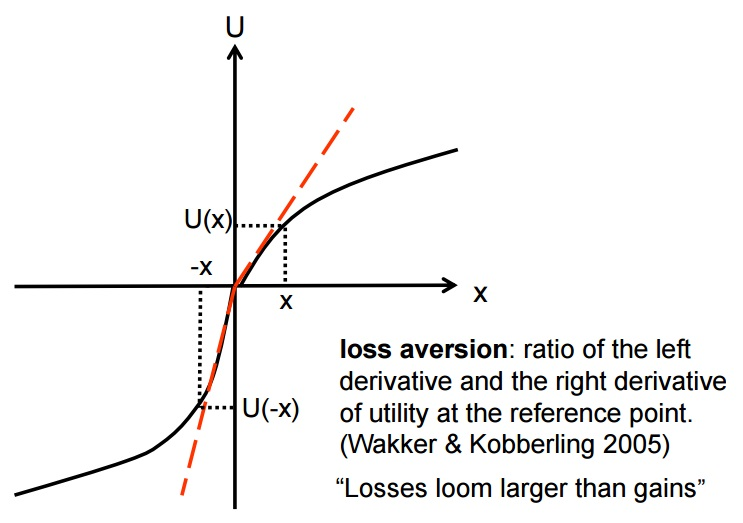
\includegraphics[width=10cm]{Figure1.png} \\

A second possible explanation that comes to the same conclusion that we do not agree with
the statement by Levy and Levy (2002) is the following:
Looking at the probability weighting of cumulative prospect theory, shows that small
probabilities are overweighted and moderate and large probabilities are underweighted (see the second graph below). 

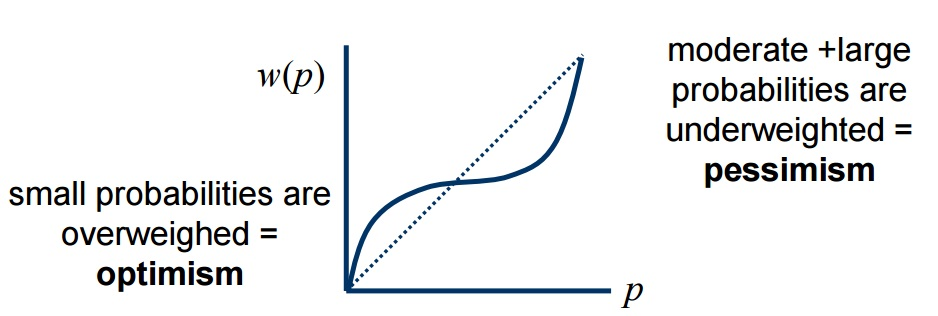
\includegraphics[width=12cm]{Figure2.png} \\

Why do people prefer E over F? In prospect F there is a small probability of a very large
negative outcome. Since it is a small probability and a negative outcome, people are
pessimistic according to CPT. Prospect E on the other hand has equal moderate probabilities
and is hence preferred over a prospect with a small overweighted outcome of loosing 6000
with probability 0.25. \\

The same logic holds for prospects G and H. In Prospect H there is a small probability of a
very large negative outcome. Since it is a small probability and a negative outcome, people
are pessimistic according to CPT and hence prefer prospect G over prospect H.

\end{document}